Miller effekt oppstår når man kobler en kondensator i feedbackloopen på en
inverterende opamp.

Kondensatorens reaktans er gitt ved:
$$X_C = \frac{1}{j\omega C} = \frac{1}{2\pi fC}$$

\begin{figure}[H]
  \caption{Kondensator i feedbackloopen}
  \centering
  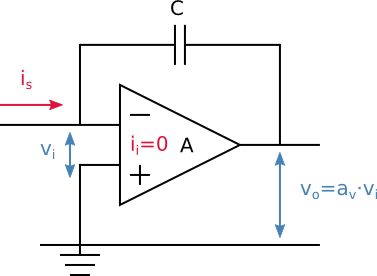
\includegraphics[width=0.5\textwidth]{./img/miller}
\end{figure}

Kondensatoren virker som om den er (1+A) ganger større enn den er.
$$i_s = \frac{v_i\cdot X_C}{v_i + A\cdot v_i}
      = \frac{X_C}{1 + A}
      = \frac{1}{j\omega C(1+A)}$$

Det gir 'millerkapasitet' $C_M$ lik:
$$C_M = C(1+A)$$

Dette betyr at høye frekvenser kuttes tidligere:
$$f_h = \frac{1}{2\pi \cdot R_{inn} \cdot C(1+A)}$$

\begin{figure}[H]
  \caption{Miller-cutoff vs vanlig cutoff}
  \centering
  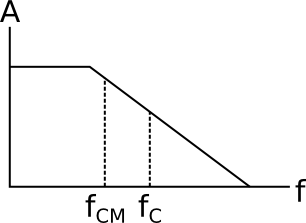
\includegraphics[width=0.5\textwidth]{./img/millercutoff}
\end{figure}
